\documentclass[12pt]{article}
\usepackage[utf8]{inputenc}
\usepackage[margin=1.2in]{geometry} 
\usepackage{graphicx}
\linespread{1.2}

\title{COUPLING OF SU2 OPEN-SOURCE COMPUTATIONAL FLUID DYNAMICS SOFTWARE WITH DEVELOPED NUMERICAL ABLATION MODEL FOR AEROSPACE APPLICATIONS}
\author{Mutlu Çelik  email}
\date{July 25, 2021}

\begin{document}

\maketitle

\section{Introduction} In aerospace engineering, computational analysis has an important role for design and analysis engineers. Therefore, there are many commercial and open sources software, which are just developed to model specific problem of aerospace engineering, available. One of the most common field called as Computational Fluid Dynamics(CFD) is highly demanded in today’s industry so that aerospace companies must pay significant amount of money(around 20,000$ to 60,000$ per license/year) for licenses of the commercial CFD software. This is a good reason for them to invest in open source software developers. 
The SU2 is a C++ based, open-source CFD software used for multi-physics simulation and design, it also has an optimization tool inside. SU2 is a common software used by CFD analysis engineers whole over the world, this is why there are many developers and contributors of it which provides a fast progress for new tools[1]. Therefore, there are many different solvers added by independent contributors in SU2 software. However, they are mostly solvers of different type of flow characteristic. The software does not have a compact thermochemical solver which models the ablation phenomenon on the surface of aerodynamic design. \newline
Thermal management is an important part of high speed vehicles like aircrafts, space shuttles and missiles so it should be considered during the aerodynamic design phase of engineering design. For high aerothermal loads, many different thermal protection systems(TPS) are developed. One easy and efficient way is to use ablative TPS materials to dissipate high entering heat flux, this is why it is one of the most common TPS for reentry missions of NASA as it is seen in Figure \ref{fig:gemini}.  Ablation simply means degradation or removing of a material surface due to chemical reactions, erosion or vaporization. There are significant studies in the literature which are presenting numerical models to model this phenomenon[3-5]. However, for open source software SU2, there are no significant effort found to model ablation with flow solvers. Therefore, adding the numerical model of this phenomenon to SU2 software is considered as an important contribution to literature. \newline
\begin{figure}[h!]
  \centering
  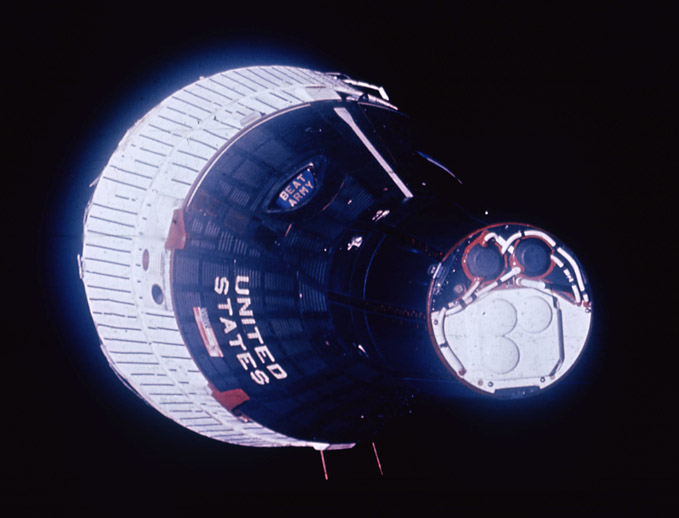
\includegraphics[width=0.8 \linewidth]{gemini_6.jpg}
  \caption{Gemini 6A spacecraft, black side is charring ablative TPS(painted)}
  \label{fig:gemini}
\end{figure}

\section{Aims, Objectives and Research Question}
The aim of this research is firstly to develop a numerical model that solves the partial differential equations of thermochemical ablation accurately and approximate the  ablative behavior of the identified charring material. For this purpose, one dimensional equations of internal energy balance, internal mass balance, surface energy balance and surface recession needs to be numerically modelled. The complexity of the phenomenon can be seen in Figure \ref{fig:char_model} , each arrow represents a part of these equations and they all need to be solved simultaneously. \newline
\begin{figure}[h!]
  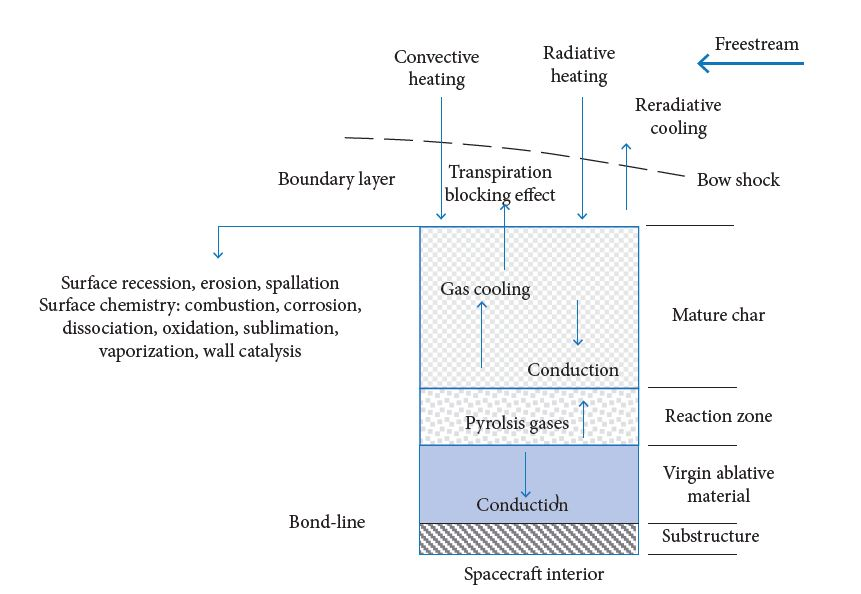
\includegraphics[width=\linewidth]{char_model.jpg}
  \caption{Shematic of charring ablative thermal protection system}
  \label{fig:char_model}
\end{figure}
SU2 software is developed based on C++ language but it has compatibility with python language and there are many tools developed based on python.  The interface of SU2 and python is targeted to investigate since the ablation numerical solver is aimed to develop based on python. On the other hand, “NEMO” the non-equilibrium models solver of SU2[6] needs to be well understood since it simulates the chemically reactive and non-equilibrium flows which is the case for ablation phenomenon. Additionally, Mutation++ thermochemistry library has to be coupled with the solver too, learning of the capabilities of this library is going to be helpful for further studies too. \newline
In the literature there are very few studies of using NEMO solver of SU2. Therefore, this study can be an important research in terms of contributing SU2-NEMO solver. In addition to this, this study could transform into a useful analysis tool for the high speed aerospace industry since it would fulfill their need of commercial software. 

\section{Methods}
The interface between the software and the ablation solver tool is based on python programming language so that it should be well studied with whole necessary libraries. Similarly, practice on Mutation++ library is needed to be able to implement it with SU2-NEMO. Before the coupling of ablation solver and SU2 software, the accuracy of the non-equilibrium flow solver is analyzed by comparing its results with experimental data and previous studies given in Bianchi’s study[3].\newline
As the numerical approach. Finite element method(FEM) is planned to be used for one dimensional numerical modelling of ablation thermochemistry while the flow is solved by SU2-NEMO solver using finite volume method. At the end, the results are going to be compared with Chen and Milos’s experimental[7] and Bianchi’s computational results[3] to see the accuracy of the ablation model. 



\begin{thebibliography}{99}
\bibitem{econ} Economon, Thomas D., Palacios, F., Copeland,S.R., Lukaczyk, T.W., Alonso,J.J
SU2: An open-source suite for multiphysics simulation and design.
Aiaa Journal 54.3 828-846, 2006.
\bibitem{Gemini}  Grimwood, J. M., et al., Project Gemini technology and operations - A chronology, NASA, NASA SP-4002, Wash., DC, 1969.
\bibitem{bian}  D. Bianchi. Modeling of Ablation Phenomena in Space Applications,
   Sapienza University of Rome, Department of Aerospace Engineering, 2007.
\bibitem{amar} Amar, Adam Joseph. 
Modeling of one-dimensional ablation with porous flow using finite control volume procedure, 2006.
\bibitem{mazz}  A. Mazzarachio.
 One-Dimensional Thermal Analysis Model for Charring Ablative Materials,
  J Aerospace Technology Management, V10,
  2018. 
\bibitem{Garbacz} Garbacz, Catarina, et al. 
Numerical Study of Shock Interference Patterns for Gas Flows with Thermal Nonequilibrium and Finite-Rate Chemistry, AIAA Scitech 2020 Forum, 2020.
\bibitem{chen} Chen, Y. K., Milos, F. S., Reda, D. C., and Stewart, D. A..
Graphite Ablation and Thermal Response Simulation under Arc-Jet Flow Conditions, AIAA Paper: 4003-4042, 2003.
\end{thebibliography}
\end{document}
